\chapter{Cadre du projet}
\label{chap:cadre_projet}

\section*{Introduction}

Ce premier chapitre a pour vocation de poser les fondements contextuels et organisationnels dans lesquels s'inscrit le projet de fin d'études. Avant de plonger dans les détails techniques et architecturaux de l'application, il est primordial de comprendre l'environnement métier, les contraintes industrielles et les défis quotidiens auxquels le Groupe COFAT fait face. Nous commencerons par la présentation de l'organisme d'accueil ainsi que le cadre général du projet. Ensuite, nous réaliserons une étude de l'existant détaillée en analysant les solutions existantes du marché ainsi que la solution historique interne. Cette analyse nous conduira à formuler une synthèse pour le choix de la solution retenue. Enfin, nous détaillerons la méthodologie de gestion de projet et de conception adoptée (Scrum/UML) pour garantir la réussite de cette réalisation.

\section{Cadre général du projet}

\subsection{Présentation de l'organisme d'accueil}
\subsubsection{Historique et cœur de métier}
Fondé en 1984, le Groupe COFAT (Compagnie Faisceaux Autos Tunisiens) est l'une des filiales phares du Groupe Elloumi, géant industriel tunisien incontournable dans le secteur de l'énergie et des composants automobiles. Depuis plus de quatre décennies, COFAT s'est spécialisé dans la conception, l'ingénierie et la fabrication de systèmes de câblage électrique et électronique pour l'industrie automobile mondiale. 

Le faisceau de câbles, souvent qualifié de \textit{système nerveux} du véhicule, est un assemblage complexe de fils conducteurs, de connecteurs, de fusibles et de gaines de protection. Il assure la distribution de l'énergie électrique et la transmission des signaux de commande entre le calculateur central et l'ensemble des organes du véhicule (éclairage, freinage ABS, sécurité airbags, système d'infodivertissement, motorisation).

Le portefeuille de produits de COFAT s'articule autour de trois grandes familles :
\begin{itemize}
    \item \textbf{Les faisceaux habitacle (Cockpit \& Body) :} Relient le tableau de bord, les portières et les équipements de confort.
    \item \textbf{Les faisceaux moteur (Engine Harnesses) :} Conçus pour résister à des environnements extrêmes (hautes températures, vibrations).
    \item \textbf{Les faisceaux haute tension (EV/PHEV) :} Développés pour répondre aux exigences des véhicules électriques et hybrides.
\end{itemize}

\subsubsection{Structure et Organigramme du Groupe COFAT}
L'organisation du Groupe COFAT s'appuie sur une direction centrale basée à Tunis (Kram) assurant la gouvernance stratégique, le pilotage financier, la politique qualité globale et les achats centraux. Sous cette direction centrale s'articulent la Direction des Opérations Industrielles, la Direction de l'Ingénierie & Méthodes, la Direction Qualité & Sécurité, et la Direction Informatique (IT).

\subsubsection{Implantation internationale et entités du Groupe}
Pour accompagner ses clients au plus près de leurs sites d'assemblage et optimiser sa compétitivité logistique, le Groupe COFAT s'est déployé à l'international. Il compte aujourd'hui 5 600 collaborateurs répartis sur 10 entités physiques majeures à travers 6 pays :
\begin{itemize}
    \item \textbf{Tunisie (Mateur \& Kairouan) :} Usines de fabrication massives (PLANT) spécialisées dans la grande série.
    \item \textbf{Tunisie (Sidi Hssin \& Kram) :} Centre de Recherche \& Développement (D\&D) et Siège administratif.
    \item \textbf{Allemagne (Gifhorn) :} Centre de support technique et d'ingénierie (D\&D) proche des constructeurs allemands.
    \item \textbf{Égypte (Le Caire) :} Usine de production (PLANT) alimentant la région Moyen-Orient et Afrique.
    \item \textbf{Mexique (Durango) :} Site industriel majeur (PLANT \& D\&D) dédié au marché nord-américain (NAFTA).
    \item \textbf{Brésil (São Paulo) :} Unité de fabrication (PLANT) pour le marché sud-américain (Mercosur).
    \item \textbf{États-Unis (El Paso, Texas) :} Bureau commercial et logistique (SERVICE).
\end{itemize}




\paragraph{Détail des 10 entités industrielles du Groupe COFAT :}
Afin d'appréhender la complexité organisationnelle du groupe, chaque site dispose de prédictions capacitaires spécifiques :
\begin{itemize}
    \item \textbf{Mateur (Tunisie) - Plant 1 \& 2 :} Spécialisés dans les faisceaux de grande série pour le groupe Volkswagen et Stellantis, comptant plus de 2 200 collaborateurs et un parc de 140 machines de coupe Komax et Schleuniger.
    \item \textbf{Kairouan (Tunisie) :} Centre industriel majeur dédié aux faisceaux moteurs et câbles haute température.
    \item \textbf{Sidi Hssin (Tunisie) :} Unité de fabrication rapide de prototypes et petites séries pour les projets en phase de démarrage (SOP - Start of Production).
    \item \textbf{Le Caire (Égypte) :} Usine d'assemblage stratégique alimentant les marchés de la zone MEA (Middle East \& Africa).
    \item \textbf{Durango (Mexique) :} Plant massif certifié IATF 16949 fournissant les chaînes de montage aux États-Unis et au Mexique.
    \item \textbf{São Paulo (Brésil) :} Centre de production latino-américain spécialisé dans les faisceaux de poids lourds (Scania, Volvo).
    \item \textbf{Gifhorn (Allemagne) \& Kram (Tunisie) :} Centres de R\&D et d'ingénierie assurant le lien direct avec les bureaux d'études des constructeurs automobiles.
\end{itemize}

\subsubsection{Management de la qualité et certifications}
Exposé aux exigences des plus grands constructeurs mondiaux (Stellantis, Volkswagen, Renault, Scania, Volvo, Daimler), COFAT applique une politique de tolérance zéro aux défauts. L'ensemble des sites du groupe est certifié selon les normes internationales les plus exigeantes : IATF 16949 (Qualité automobile), ISO 9001 (Management de la qualité), ISO 14001 (Management environnemental) et ISO 45001 (Santé et sécurité au travail).

Ces exigences de certification imposent une traçabilité rigoureuse de l'ensemble des décisions industrielles ayant un impact sur la capacité de production et les investissements en équipements.

\subsection{Contexte et Objectifs du projet}
La gestion de la capacité de production à l'échelle d'un groupe multi-sites représentait un défi opérationnel majeur. L'anticipation des besoins en machines, en surfaces au sol et en ressources humaines pour les nouveaux projets automobiles (tels que le lancement du VW Tayron ou du Stellantis J4U) exigeait une visibilité temps réel.

Les objectifs majeurs assignés au projet \textit{Cofat Capacity Study} sont :
\begin{enumerate}
    \item \textbf{Centraliser et sécuriser} l'ensemble des données de capacité sur un portail web unique avec contrôle d'accès RBAC.
    \item \textbf{Automatiser la saisie} via un moteur d'importation de fichiers Excel locaux utilisé par les Site Managers.
    \item \textbf{Consolider instantanément} les besoins mondiaux en équipements, surfaces et effectifs RH pour le siège.
    \item \textbf{Numériser le workflow} des demandes de budget non-industriel entre les usines et le département Achats central.
\end{enumerate}

\section{Étude de l'existant}
Afin de fonder scientifiquement notre démarche de développement et de justifier le choix d'un système sur mesure, nous avons réalisé une étude approfondie de trois solutions existantes du marché ainsi que du processus manuel historique interne.

\subsection{Étude du système ERP SAP}
\begin{itemize}
    \item \textbf{Description :} SAP ERP (module Production Planning / Capacity Requirements Planning) est un système de gestion d'entreprise lourd utilisé dans les grandes industries pour planifier les ordres de fabrication à partir des gammes opératoires. La Figure \ref{fig:existant_sap} illustre une vue transactionnelle typique du module de charge capacitaire SAP.
    \item \textbf{Avantages :} Excellente intégrité transactionnelle, lien direct avec la comptabilité et la gestion des stocks.
    \item \textbf{Limites pour COFAT :} Extrêmement coûteux en licences et complexe à paramétrer pour 10 sites internationaux distants. Il s'avère trop rigide pour la planification agile des projets automobiles futurs et ne permet pas l'import souple de tableurs Excel de travail. Il n'offre aucun workflow spécifique pour le budget non-industriel.
\end{itemize}

\begin{figure}[H]
    \centering
    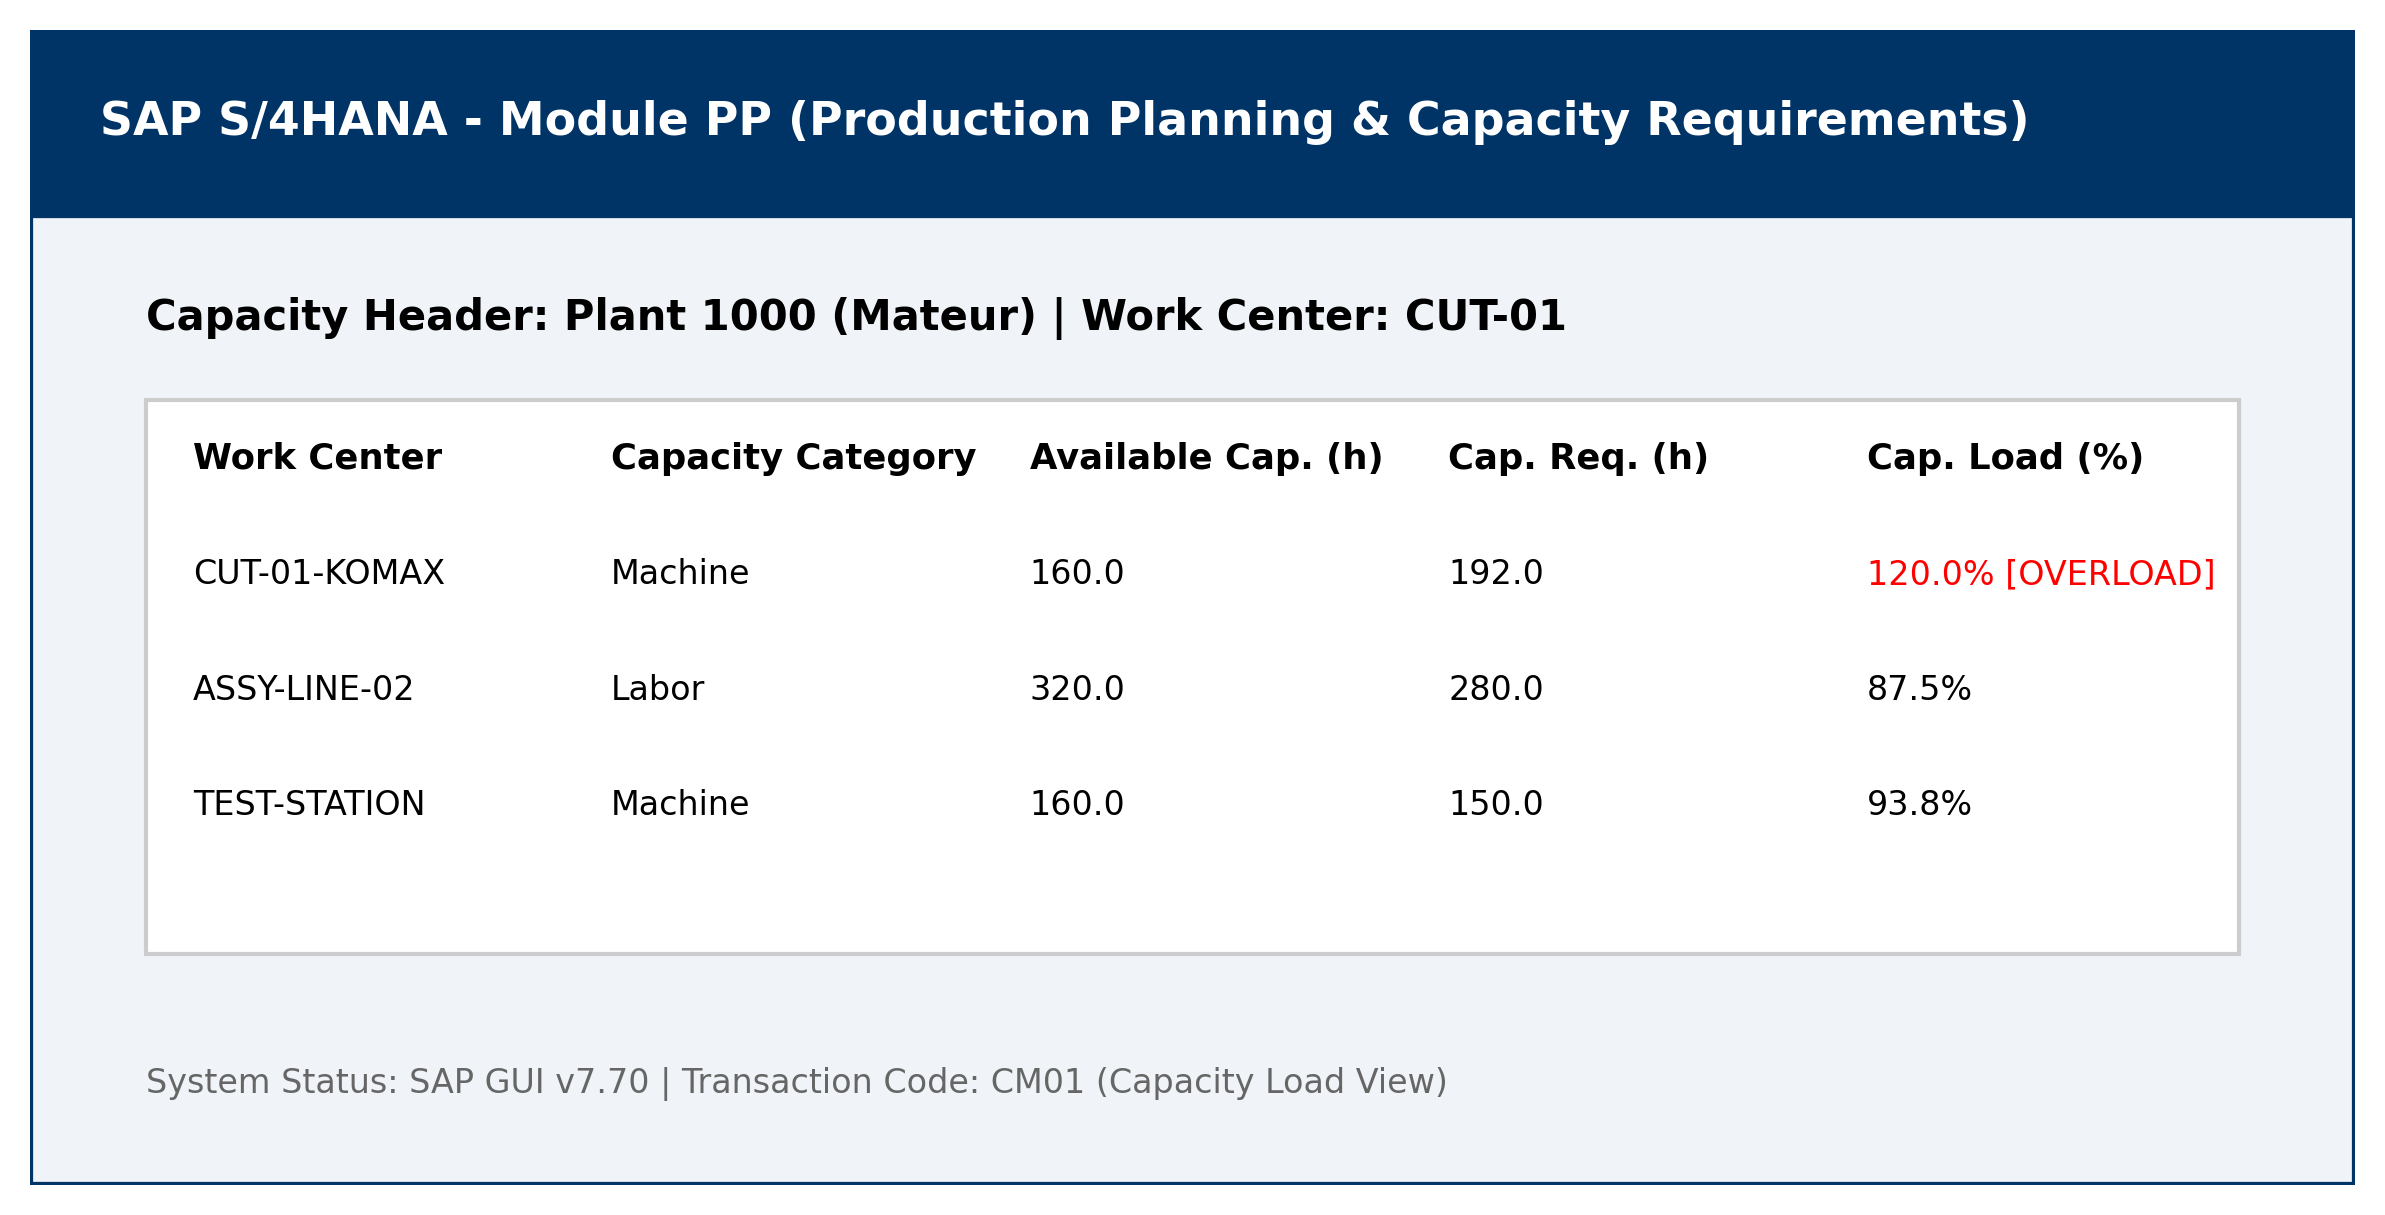
\includegraphics[width=0.85\textwidth]{img/existant_sap.png}
    \caption{Interface d'analyse de charge du module SAP ERP Production Planning}
    \label{fig:existant_sap}
\end{figure}

\subsection{Étude de l'outil d'ordonnancement Preactor APS}
\begin{itemize}
    \item \textbf{Description :} Siemens Opcenter APS (Preactor) est une solution spécialisée dans l'ordonnancement détaillé et la planification à capacité finie sur les lignes de production à court terme. La Figure \ref{fig:existant_preactor} présente un diagramme de Gantt d'ordonnancement machine généré par cet outil.
    \item \textbf{Avantages :} Optimisation fine des séquences de passage des machines et simulation des goulots d'étranglement en atelier.
    \item \textbf{Limites pour COFAT :} Focalisé uniquement sur le suivi très court terme des machines, cet outil n'offre ni la gestion des surfaces d'usine (Espaces), ni la projection temporelle à 3 ans des effectifs RH, ni la budgétisation collaborative transversale.
\end{itemize}

\begin{figure}[H]
    \centering
    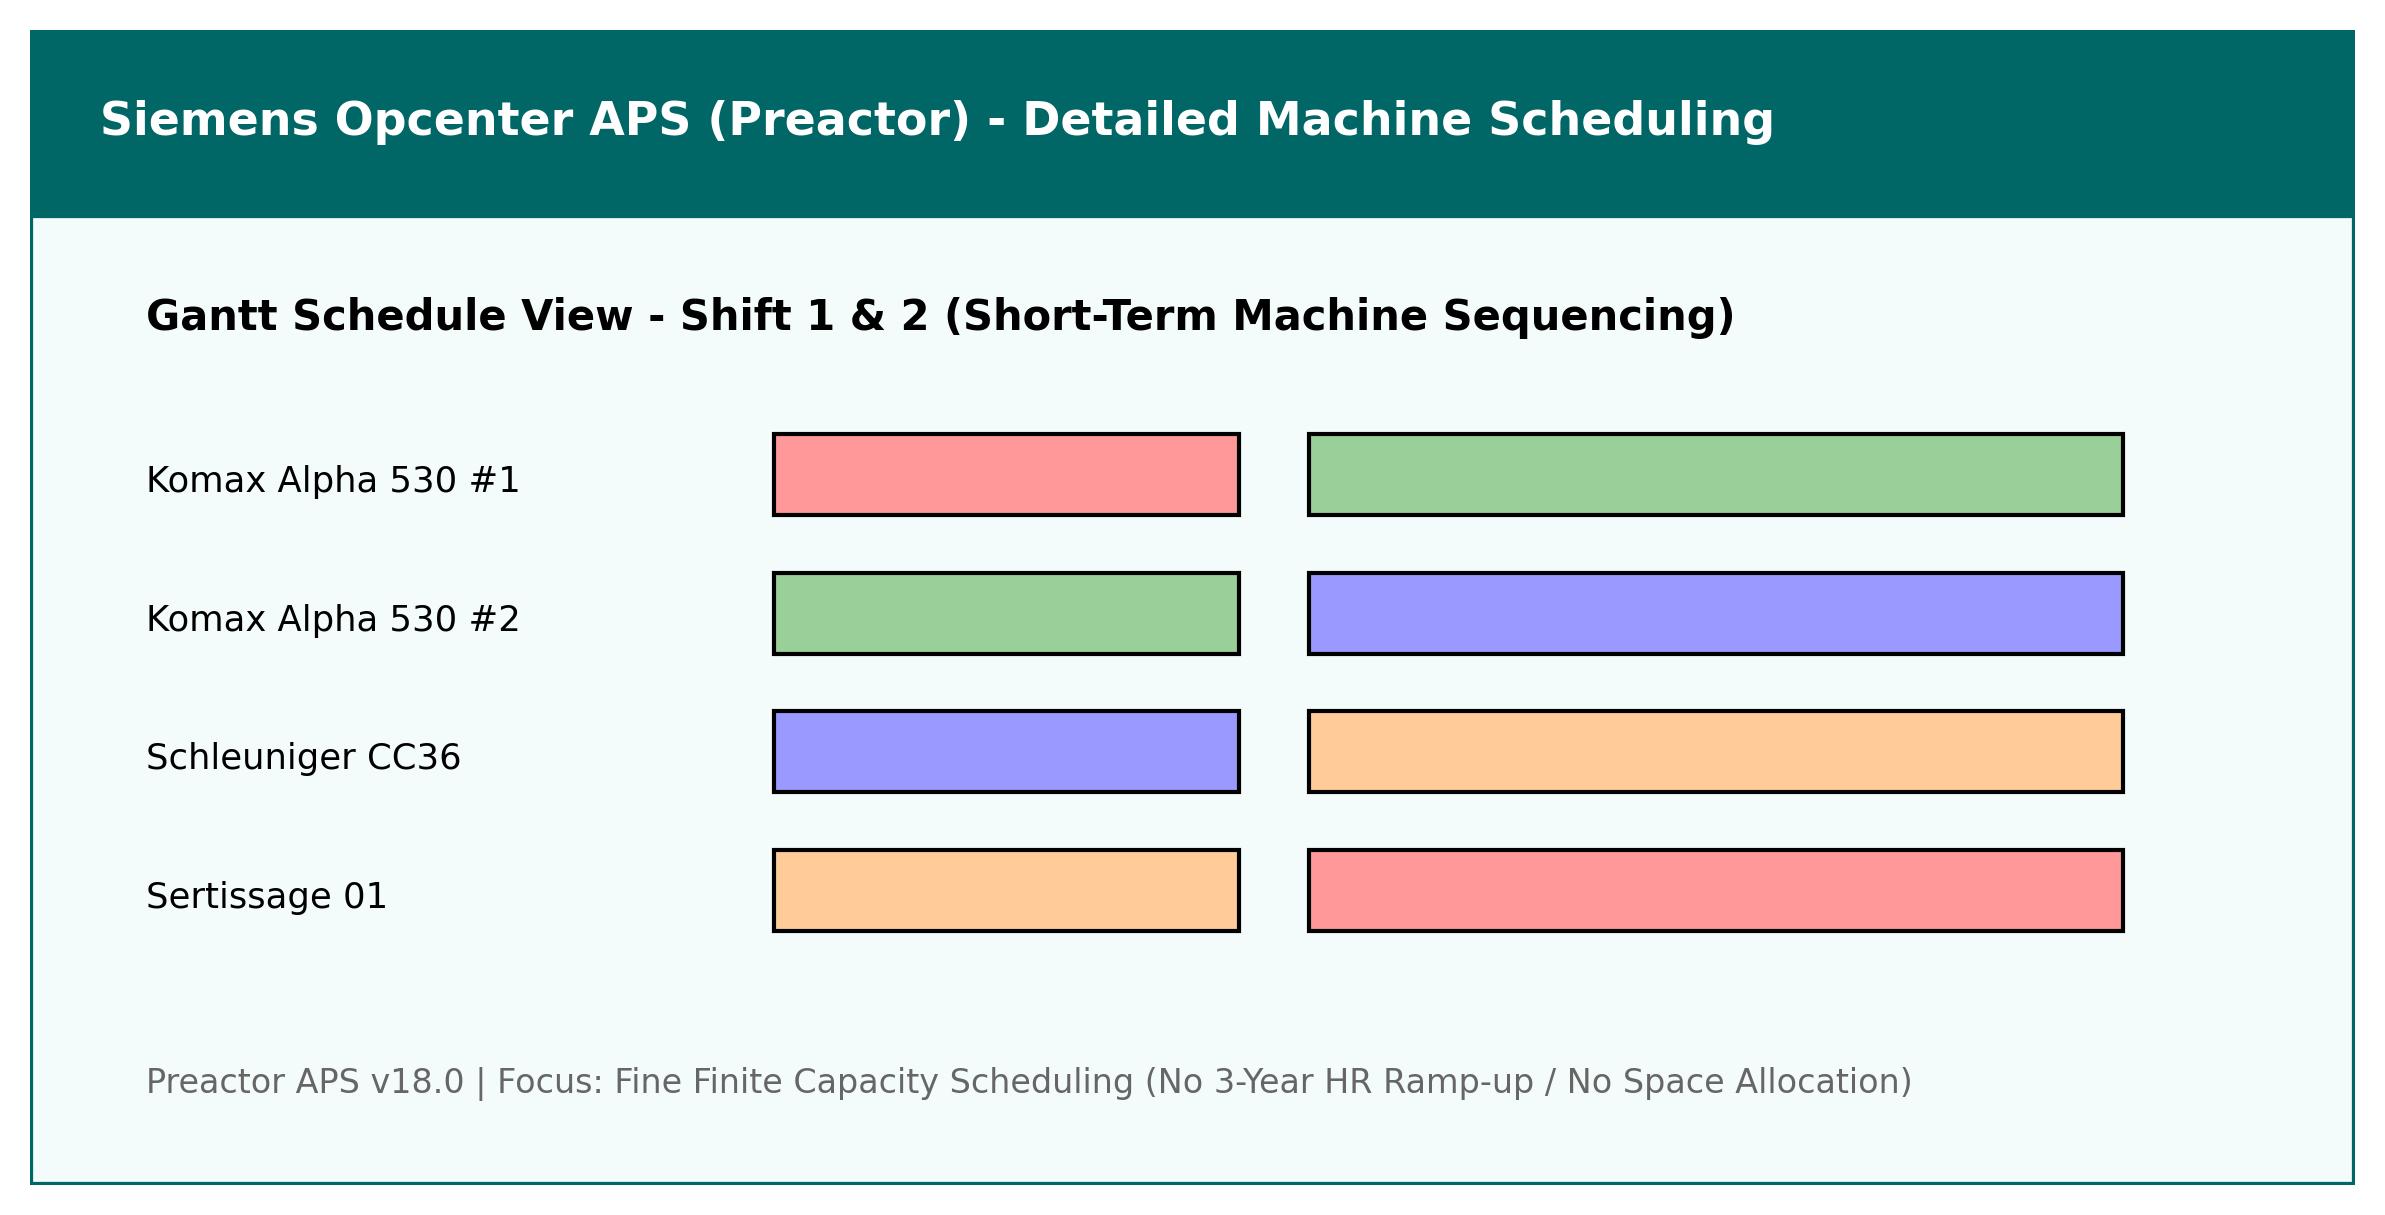
\includegraphics[width=0.85\textwidth]{img/existant_preactor.png}
    \caption{Interface d'ordonnancement court terme sous Siemens Opcenter APS (Preactor)}
    \label{fig:existant_preactor}
\end{figure}

\subsection{Étude du système historique Excel COFAT}
\begin{itemize}
    \item \textbf{Description :} La solution historique interne utilisée chez COFAT avant ce projet, reposant sur la saisie locale dans des tableurs Excel isolés (Équipements, Espaces, RH) et leur transmission par courriel au siège pour consolidation manuelle. La Figure \ref{fig:existant_excel} montre un exemple de tableur Excel de travail utilisé sur le site de Mateur.
    \item \textbf{Avantages :} Souplesse perçue par l'utilisateur local, aucun coût de licence directe.
    \item \textbf{Limites pour COFAT :} Risques élevés d'erreurs de copier-coller et de formules corrompues, absence de contrôle d'accès sécurisé (RBAC), perte de traçabilité lors des audits IATF 16949, et temps de consolidation mondiale très long (plusieurs jours/semaines).
\end{itemize}

\begin{figure}[H]
    \centering
    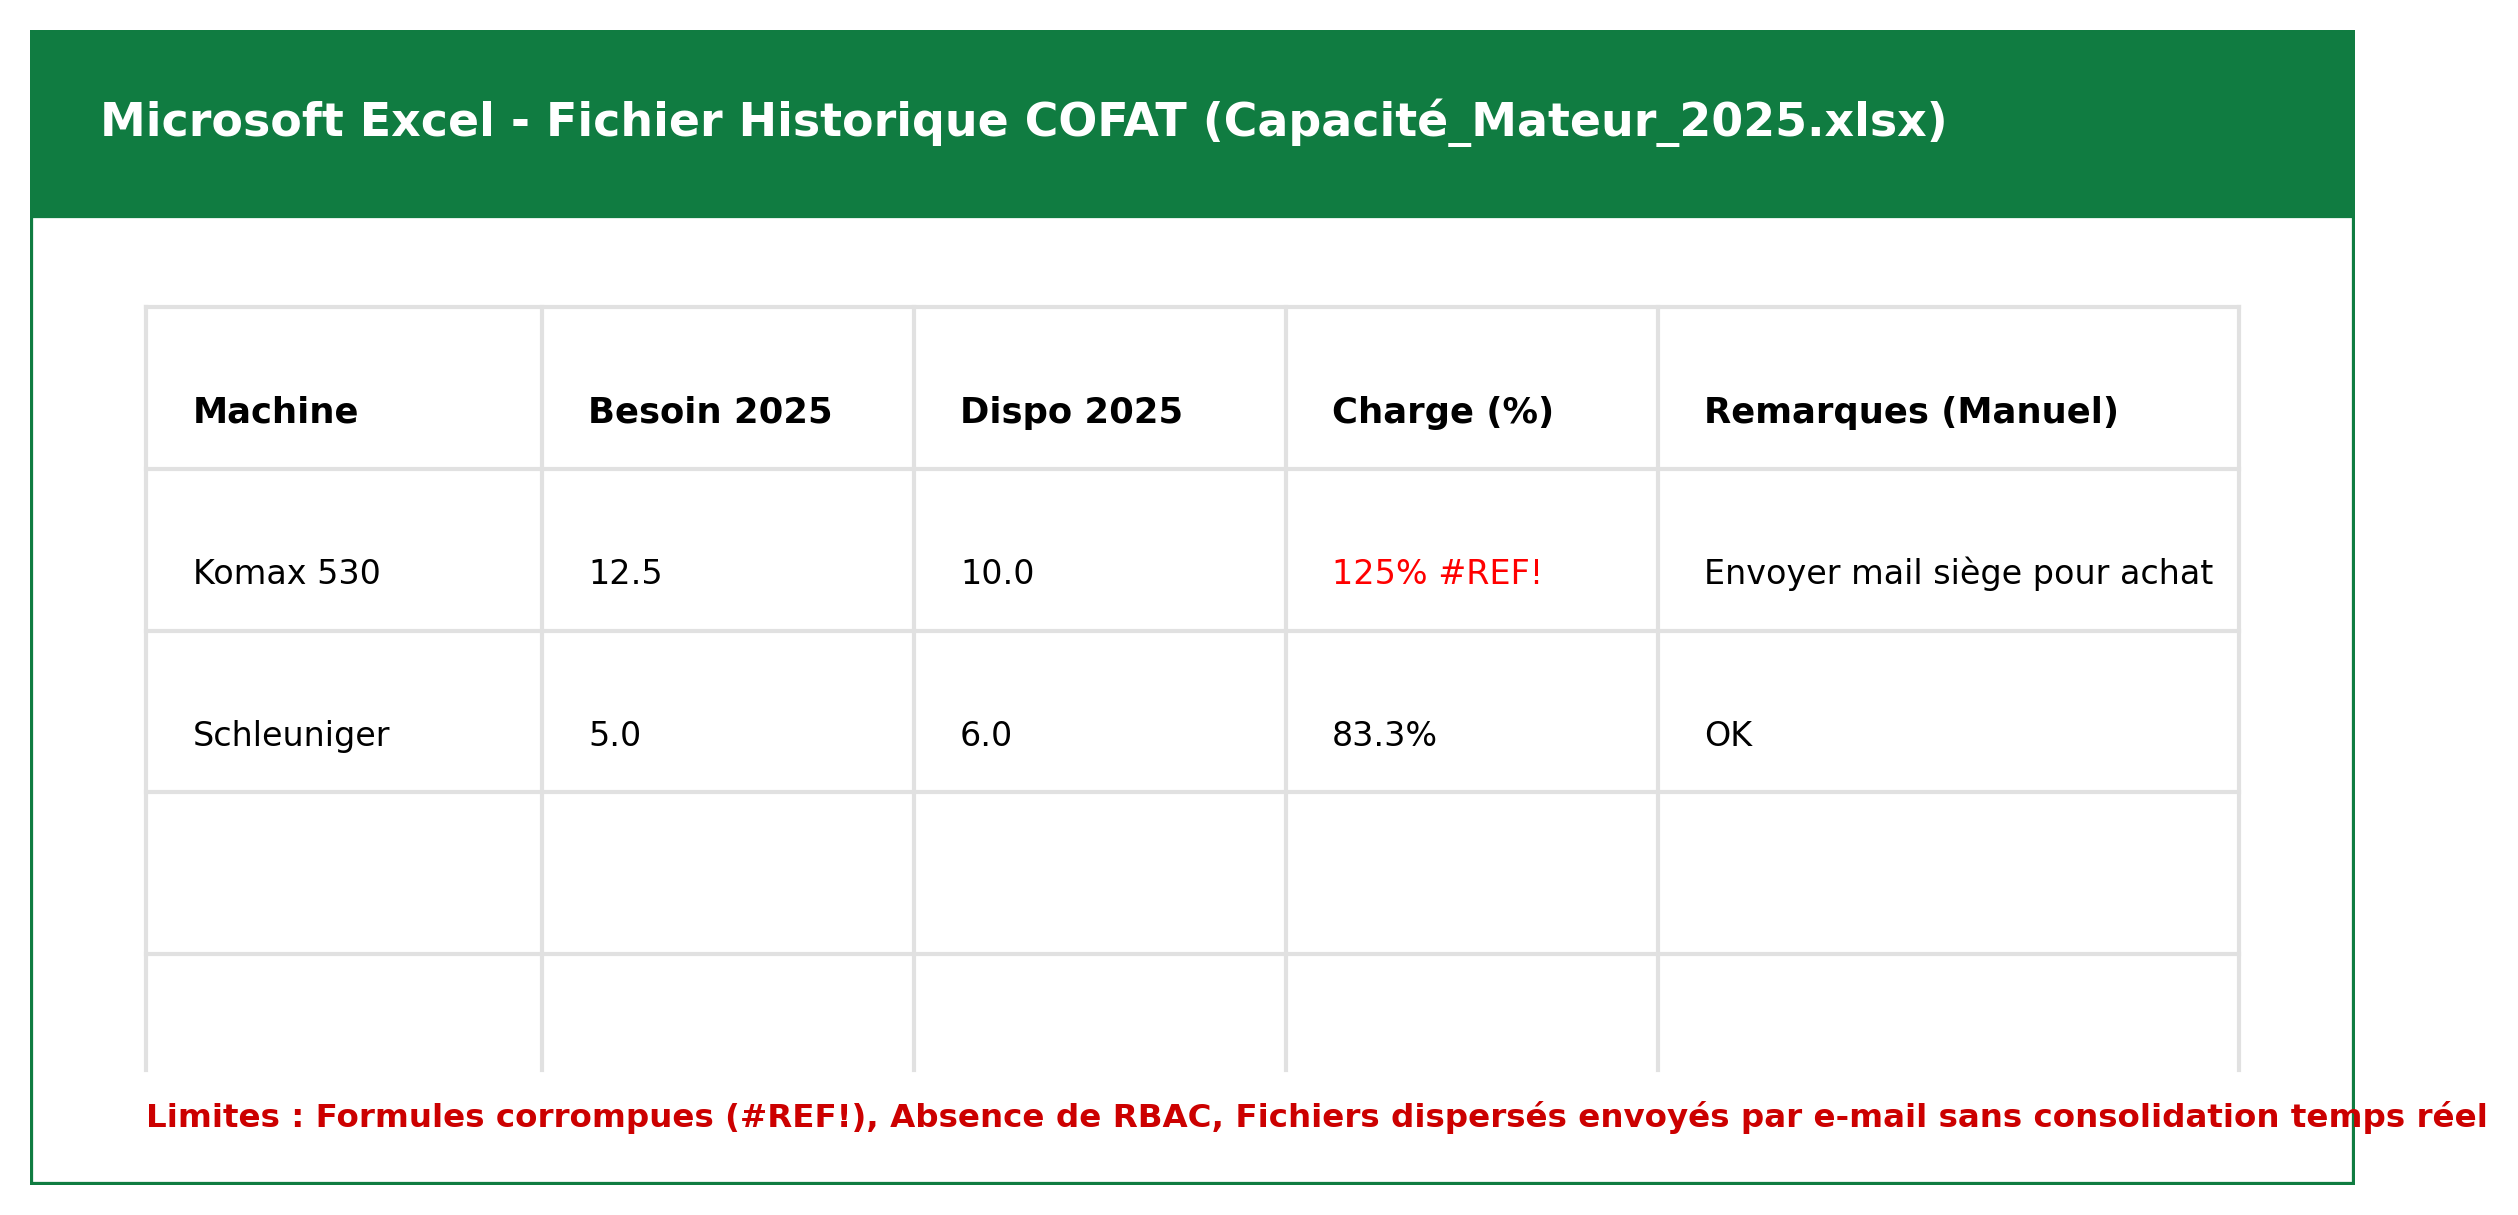
\includegraphics[width=0.85\textwidth]{img/existant_excel.png}
    \caption{Tableur Excel historique de gestion capacitaire utilisé chez COFAT}
    \label{fig:existant_excel}
\end{figure}

\section{Synthèse pour le choix de la solution}
Le Tableau \ref{tab:synthese_solution} présente la synthèse comparative de ces trois solutions existantes par rapport aux exigences cibles de la plateforme \textit{Cofat Capacity Study}.

\begin{table}[h]
\centering
\begin{tabular}{|p{3.5cm}|p{3cm}|p{3cm}|p{3cm}|p{3.5cm}|}
\hline
\textbf{Critère d'évaluation} & \textbf{Solution 1 (SAP ERP)} & \textbf{Solution 2 (Siemens APS)} & \textbf{Solution 3 (Excel / Mails)} & \textbf{\textit{Cofat Capacity Study}} \\ \hline
Planification Équipements & Oui (lourd) & Oui (très détaillé) & Oui (local isolé) & \textbf{Oui (agile + import Excel)} \\ \hline
Gestion des Espaces & Non & Non & Partielle (manuel) & \textbf{Oui (surfaces et zones)} \\ \hline
Prévision RH (3 ans) & Non & Non & Partielle (manuel) & \textbf{Oui (matrice temporelle)} \\ \hline
Consolidation Mondiale & Complexe & Non & Très lente / manuelle & \textbf{Instantanée (temps réel)} \\ \hline
Workflow Budget Non-Ind. & Non & Non & Inexistant & \textbf{Oui (Achat / Site Mgr)} \\ \hline
Sécurité et RBAC & Très élevée & Élevée & Faible (fichiers) & \textbf{Élevée (JWT / HttpOnly)} \\ \hline
Coût d'implémentation & Très élevé & Élevé & Faible & \textbf{Optimisé (Interne PFE)} \\ \hline
\end{tabular}
\caption{Synthèse comparative des solutions existantes face aux besoins de COFAT}
\label{tab:synthese_solution}
\end{table}

Cette synthèse démontre la pertinence du développement d'une application web 3-tiers dédiée sur mesure, combinant la souplesse de l'importation Excel pour les usines et la puissance de la consolidation centralisée en temps réel pour le siège.

\section{Méthodologie de gestion de projet à adopter}

\subsection{Méthodologie de SCRUM}
Nous recherchons toujours la méthode la plus efficace et la plus rapide de mettre en œuvre notre projet. Pour cela, nous utilisons des méthodes agiles. Scrum est le cadre agile le plus simple. Scrum garantit la meilleure vue d'ensemble de notre projet et vise à réduire les difficultés, telles que le manque de planification, le travail est effectué à travers un cycle court appelé Sprint. Dans un Sprint, notre équipe travaille à partir d'une liste d'éléments appelée \textit{Backlog}.

Nous avons choisi la méthodologie SCRUM qui fait partie de la méthodologie Agile pour différentes raisons parmi lesquelles :
\begin{itemize}
    \item La transparence.
    \item La tolérance aux différents changements.
    \item Les besoins ne sont pas totalement figés au départ et s'affinent au fur et à mesure des retours métier.
    \item La présence de réunions régulières (Daily Scrum, Sprint Review) qui permettent de bien résoudre les problèmes et de trouver des solutions rapidement.
\end{itemize}

La Figure \ref{fig:scrum_process} représente le parcours et le cycle de vie de la méthodologie SCRUM.

\begin{figure}[H]
    \centering
    \includegraphics[width=0.75\textwidth]{img/Scrum-process.png}
    \caption{Cycle de vie de la méthodologie SCRUM}
    \label{fig:scrum_process}
\end{figure}

\subsection{Les rôles dans SCRUM}
La méthodologie agile SCRUM implique trois rôles principaux qui sont :
\begin{itemize}
    \item \textbf{Product Owner : (M. Said Bouchouicha)} -- C'est le représentant des clients et des utilisateurs finaux, et c'est lui qui est l'expert métier de l'équipe au sein de COFAT. C'est à lui de définir et prioriser la liste des fonctionnalités du produit (Product Backlog) et d'effectuer l'analyse nécessaire pour la prise de décision.
    \item \textbf{Scrum Master : (M. Mohamed Alouani)} -- C'est le garant de la méthodologie SCRUM. Il s'assure que tout le monde peut maximiser ses capacités en éliminant les obstacles et en protégeant l'équipe des perturbations externes. Par ailleurs, il garantit que l'équipe chargée du projet adopte fidèlement les principes et les valeurs de SCRUM.
    \item \textbf{Équipe : (Sayf Eddine Zakraoui)} -- L'équipe rassemble tous les rôles généralement nécessaires à un projet (analyse, conception, développement frontend/backend et tests), elle est organisée et reste inchangée pendant la durée d'un sprint.
\end{itemize}

\subsection{Méthodologie de conception à adopter}
La modélisation du système d'information a pour but de permettre aux entreprises de communiquer avec des services ou des entreprises spécialisées dans l'informatique et de décrire leurs opérations et leurs besoins. Le modèle peut être résumé de manière claire et compréhensible pour tout le monde.

Pour cela, nous avons choisi le langage de modélisation UML (\textit{Unified Modeling Language}), car il s'appuie sur la standardisation et pour la diversité de ses diagrammes. Ce qui permet de réaliser une analyse détaillée des besoins, des vues statiques (diagrammes de cas d'utilisation, diagramme de classes) et des vues dynamiques (diagrammes de séquence).

\section*{Conclusion}
Dans ce chapitre, nous avons présenté le projet dans son cadre général, nous passons maintenant à la spécification des besoins.
